\documentclass[a4paper,12pt]{article}
	
\usepackage[T2A]{fontenc}			
\usepackage[utf8]{inputenc}			
\usepackage[english,russian]{babel}	

\usepackage[
bookmarks=true, colorlinks=true, unicode=true,
urlcolor=black,linkcolor=black, anchorcolor=black,
citecolor=black, menucolor=black, filecolor=black,
]{hyperref}

\usepackage{color}
\usepackage{caption}


\usepackage{amsmath,amsfonts,amssymb,amsthm,mathtools} 
\usepackage{wasysym}

\usepackage{graphicx}
%\usepackage[cache=false]{minted}
\usepackage{cmap}
\usepackage{indentfirst}

\usepackage{listings} 
\usepackage{fancyvrb}
\usepackage{slashbox}

\usepackage{geometry}
\geometry{left=2cm}
\geometry{right=1.5cm}
\geometry{top=1cm}
\geometry{bottom=2cm}

\setlength{\parindent}{5ex}
\setlength{\parskip}{0.5em}

\usepackage{titlesec}
\usepackage{pgfplots}
\usepackage{filecontents}
\usetikzlibrary{datavisualization}
\usetikzlibrary{datavisualization.formats.functions}

\DeclareCaptionFont{white}{\color{white}}
\DeclareCaptionFormat{listing}{\colorbox{gray}{\parbox{\textwidth}{#1#2#3}}}
\captionsetup[lstlisting]{format=listing,labelfont=white,textfont=white}
\lstloadlanguages{% Check Dokumentation for further languages ...
C,
C++,
csh,
Java
}

\definecolor{red}{rgb}{0.6,0,0} % for strings
\definecolor{blue}{rgb}{0,0,0.6}
\definecolor{green}{rgb}{0,0.8,0}
\definecolor{cyan}{rgb}{0.0,0.6,0.6}

\lstset{ %
language=Lisp,                 % выбор языка для подсветки
basicstyle=\small\sffamily, % размер и начертание шрифта для подсветки кода
numbers=left,               % где поставить нумерацию строк (слева\справа)
numberstyle=\tiny,           % размер шрифта для номеров строк
stepnumber=1,                   % размер шага между двумя номерами строк
numbersep=5pt,                % как далеко отстоят номера строк от подсвечиваемого кода
showspaces=false,
backgroundcolor=\color{white},         
showstringspaces=false,      % показывать или нет пробелы в строках
showtabs=false,             % показывать или нет табуляцию в строках
frame=single,              % рисовать рамку вокруг кода
tabsize=2,                 % размер табуляции по умолчанию равен 2 пробелам
captionpos=t,              % позиция заголовка вверху [t] или внизу [b] 
breaklines=true,           % автоматически переносить строки (да\нет)
breakatwhitespace=false, % переносить строки только если есть пробел
escapeinside={\%*}{*)}
}

% Для измененных титулов глав:
\definecolor{gray75}{gray}{0.75} % определяем цвет
\newcommand{\hsp}{\hspace{20pt}} % длина линии в 20pt
% titleformat определяет стиль
\titleformat{\chapter}[hang]{\Huge\bfseries}{\thechapter\hsp\textcolor{gray75}{|}\hsp}{0pt}{\Huge\bfseries}

\begin{document}
	
\begin{figure}[h!]
	\begin{center}
		{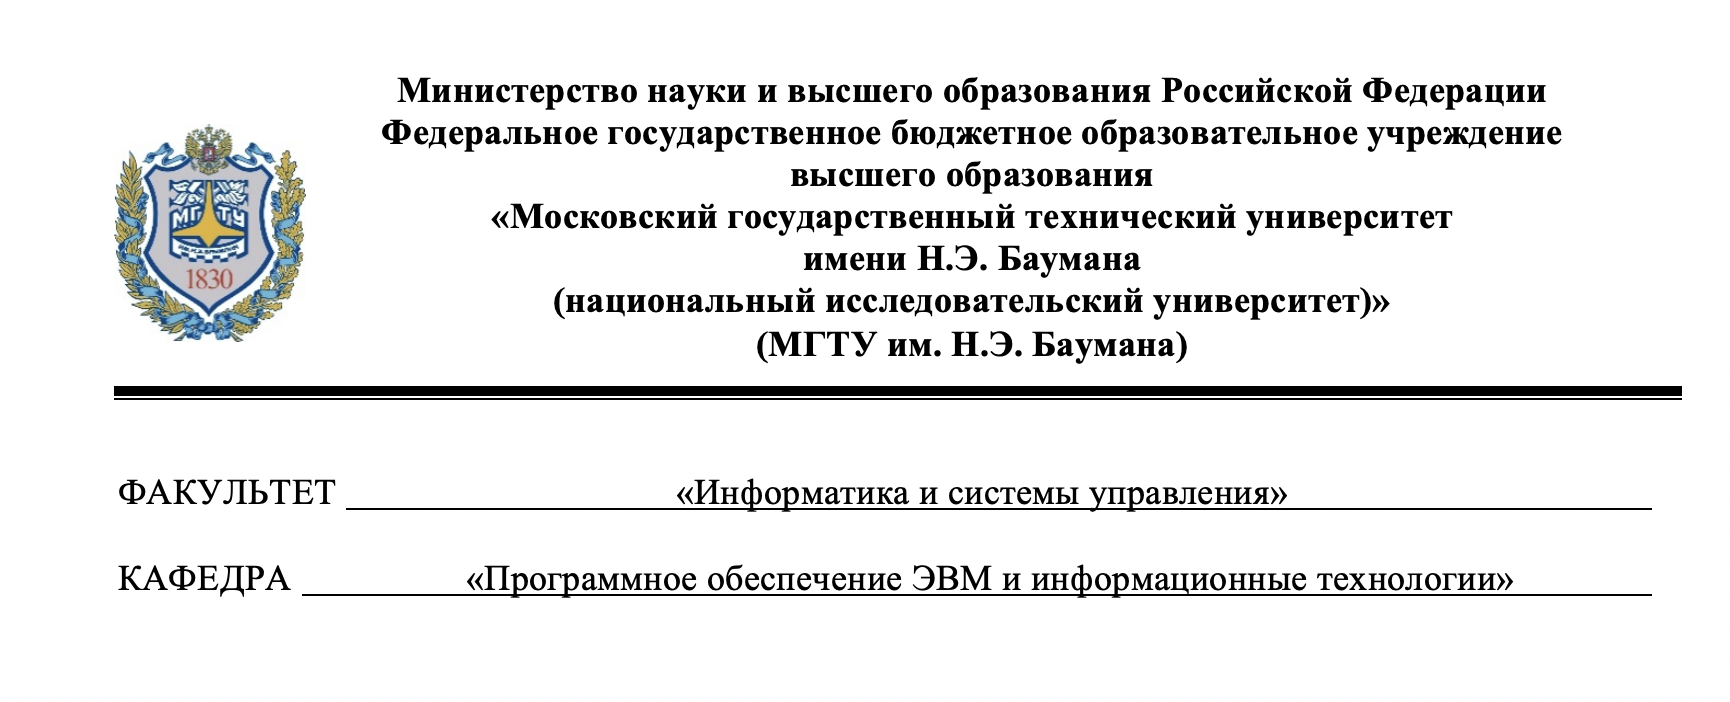
\includegraphics[width = \textwidth]{titul.png}}
	\end{center}
\end{figure}

\vspace*{20mm}

\huge
\begin{center}
	Лабораторная работа №1
\end{center}


\vspace*{50mm}

\large
\begin{flushleft}
	Студент: Луговой Д.М. \\
	Группа: ИУ7-61Б \\
	Преподаватель: Толпинская Н.Б.
\end{flushleft}

\vspace*{60mm}

\large
\begin{center}
	Москва, 2020 г.
\end{center}

\thispagestyle{empty}

\newpage
\vspace*{10mm}
\textbf{Цель работы}: приобрести навыки использования списков и стандартных функций Lisp.\\

\textbf{Задачи работы}: изучить способ использования списков для фиксации информации, внутреннее представление одноуровневых и структурированных списков, методы их обработки с использованием базовых функций Lisp.
\begin{enumerate}
\item \textbf{Базовые элементы языка}

Функциональное программирование ориентировано на символьную обработку данных. 

Базис в Lisp образуют атомы, структуры, базовые функции, базовые функционалы.

Данные и программы в Lisp представлены в виде символьных выражений - S-выражений. Любое S-выражение является атомом или структурой.

Атомы в Lisp:
\begin{itemize}
\item Символы - последовательность из букв и цифр, начинающаяся с буквы, включая и другие литеры, не занятые в синтаксисе.
\item Специальные символы - логические константы T и Nil.
\item Самовычислимые атомы - натуральные, дробные и вещественные числа и строки.
\end{itemize}

Более сложные данные выстраиваются из структур данных - одинаково устроенных блоков памяти. В Lisp это бинарные узлы, содержащие пары объектов произвольного вида. Любая структура в Lisp заключается в круглые скобки.

Точечная пара представляет собой бинарный узел, левая и правая части которого равноправны и могут хранить в себе атомы и точечные пары, разделенные точкой(Примеры: (A.B), (A.(C.D)))

\item \textbf{Определение списка, его синтаксис}

Список – это структура данных. Может быть пустой и непустой. Список может быть пустым. В  Lisp возможны два типа представления пустого списка: пара пустых скобок и специальный символ Nil. Синтаксически списком является последовательность из нуля или более элементов, заключенных в скобки и разделенных пробелами.(Пример: (A B C), (A), (A (B)))

\newpage
\item \textbf{Функция QUOTE и символ '}

И программа, и данные в Lisp представляются в списочной форме. Для явного выделения данных используется функция QUOTE и ' - ее сокращенное обозначение. Эта функция защищяет выражение от вычисления.

\item \textbf{Представление списка в памяти}

В памяти список представлен списочной ячейкой, содержащей указатели на голову списка и на его хвост. Голова списка представляет из себя S-выражение, хвост является списком.\\

\end{enumerate}

{\LARGE Задание №1}\\

Представить списки в виде списочных ячеек:
\begin{itemize}
\item '(open close half)
\begin{figure}[ht!]
\center{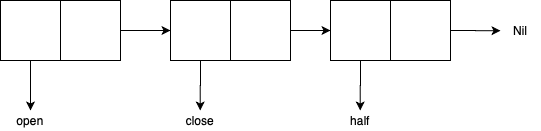
\includegraphics[scale=0.6]{FaLP1.png}}
\end{figure}
\item '((open1)(close2)(half3))
\begin{figure}[ht!]
\center{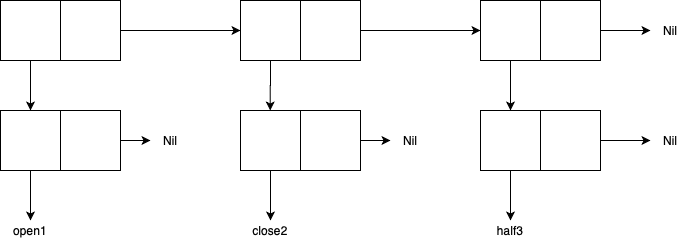
\includegraphics[scale=0.6]{FaLP2.png}}
\end{figure}
\newpage
\item '((one) for all (and(me(for you))))
\begin{figure}[ht!]
\center{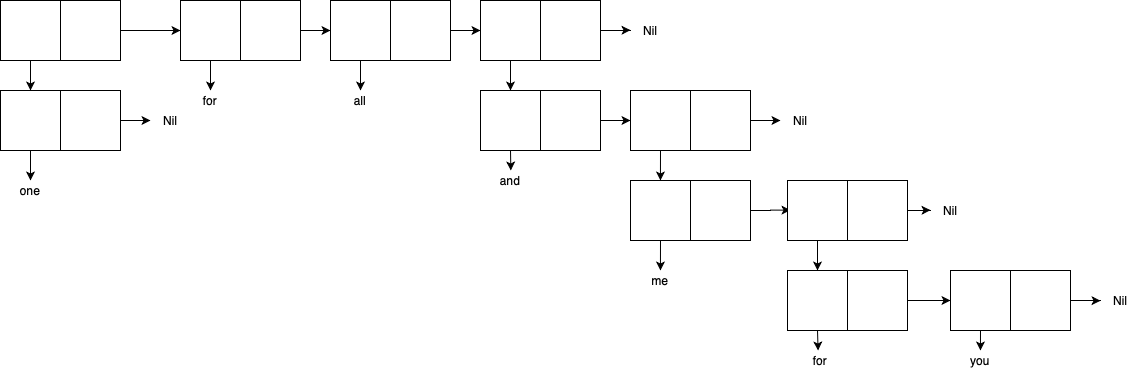
\includegraphics[scale=0.45]{FaLP3.png}}
\end{figure}
\item '((TOOL)(call))
\begin{figure}[ht!]
\center{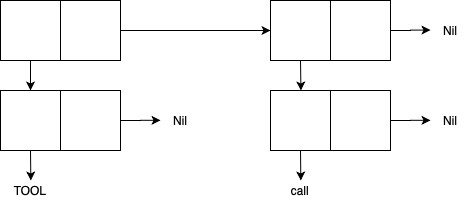
\includegraphics[scale=0.6]{FaLP4.png}}
\end{figure}
\item '((TOOL1)((call2))((sell)))
\begin{figure}[ht!]
\center{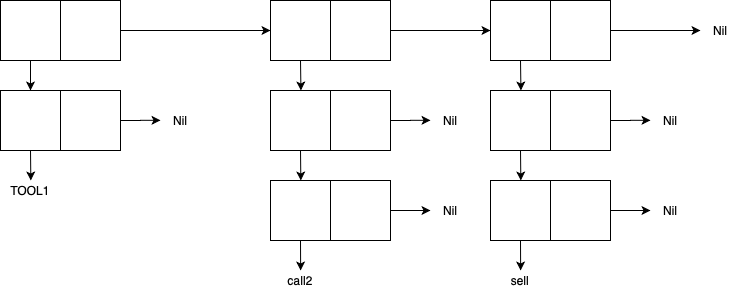
\includegraphics[scale=0.6]{FaLP5.png}}
\end{figure}
\newpage
\item '(((TOOL)(call))((sell)))
\begin{figure}[ht!]
\center{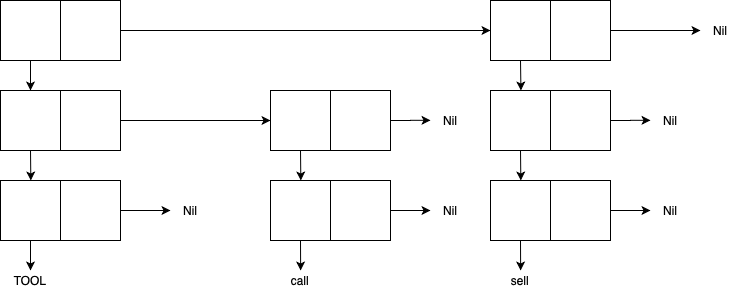
\includegraphics[scale=0.6]{FaLP6.png}}
\end{figure}
\end{itemize}

{\LARGE Задание №2}\\

Используя только функции CAR и CDR, написать выражения, возвращающие:
\begin{enumerate}
\item второй элемент списка

(car (cdr '(1 2 3 4)))\\
Пример: (car (cdr '((1 2) 3 (4 (5))))) -> 3
\item третий элемент списка


(car (cdr (cdr '(1 2 3 4))))\\
Пример: (car (cdr (cdr '(1 (2 (3)) ((4) 5 (6))) 7)))) -> ((4) 5 (6))

\item четвертый элемент списка

(car (cdr (cdr (cdr '(1 2 3 4)))))\\
Пример: (car (cdr (cdr (cdr '(((1 2) ((3 4) 5)) 6 (7 8) ((10) 11)))))) -> \\ -> ((10) 11)

\end{enumerate}

\end{document}

